\documentclass[twoside]{book}

% Packages required by doxygen
\usepackage{fixltx2e}
\usepackage{calc}
\usepackage{doxygen}
\usepackage[export]{adjustbox} % also loads graphicx
\usepackage{graphicx}
\usepackage[utf8]{inputenc}
\usepackage{makeidx}
\usepackage{multicol}
\usepackage{multirow}
\PassOptionsToPackage{warn}{textcomp}
\usepackage{textcomp}
\usepackage[nointegrals]{wasysym}
\usepackage[table]{xcolor}

% NLS support packages
\usepackage{polski}
\usepackage[T1]{fontenc}

% Font selection
\usepackage[T1]{fontenc}
\usepackage[scaled=.90]{helvet}
\usepackage{courier}
\usepackage{amssymb}
\usepackage{sectsty}
\renewcommand{\familydefault}{\sfdefault}
\allsectionsfont{%
  \fontseries{bc}\selectfont%
  \color{darkgray}%
}
\renewcommand{\DoxyLabelFont}{%
  \fontseries{bc}\selectfont%
  \color{darkgray}%
}
\newcommand{\+}{\discretionary{\mbox{\scriptsize$\hookleftarrow$}}{}{}}

% Page & text layout
\usepackage{geometry}
\geometry{%
  a4paper,%
  top=2.5cm,%
  bottom=2.5cm,%
  left=2.5cm,%
  right=2.5cm%
}
\tolerance=750
\hfuzz=15pt
\hbadness=750
\setlength{\emergencystretch}{15pt}
\setlength{\parindent}{0cm}
\setlength{\parskip}{3ex plus 2ex minus 2ex}
\makeatletter
\renewcommand{\paragraph}{%
  \@startsection{paragraph}{4}{0ex}{-1.0ex}{1.0ex}{%
    \normalfont\normalsize\bfseries\SS@parafont%
  }%
}
\renewcommand{\subparagraph}{%
  \@startsection{subparagraph}{5}{0ex}{-1.0ex}{1.0ex}{%
    \normalfont\normalsize\bfseries\SS@subparafont%
  }%
}
\makeatother

% Headers & footers
\usepackage{fancyhdr}
\pagestyle{fancyplain}
\fancyhead[LE]{\fancyplain{}{\bfseries\thepage}}
\fancyhead[CE]{\fancyplain{}{}}
\fancyhead[RE]{\fancyplain{}{\bfseries\leftmark}}
\fancyhead[LO]{\fancyplain{}{\bfseries\rightmark}}
\fancyhead[CO]{\fancyplain{}{}}
\fancyhead[RO]{\fancyplain{}{\bfseries\thepage}}
\fancyfoot[LE]{\fancyplain{}{}}
\fancyfoot[CE]{\fancyplain{}{}}
\fancyfoot[RE]{\fancyplain{}{\bfseries\scriptsize Wygenerowano przez Doxygen }}
\fancyfoot[LO]{\fancyplain{}{\bfseries\scriptsize Wygenerowano przez Doxygen }}
\fancyfoot[CO]{\fancyplain{}{}}
\fancyfoot[RO]{\fancyplain{}{}}
\renewcommand{\footrulewidth}{0.4pt}
\renewcommand{\chaptermark}[1]{%
  \markboth{#1}{}%
}
\renewcommand{\sectionmark}[1]{%
  \markright{\thesection\ #1}%
}

% Indices & bibliography
\usepackage{natbib}
\usepackage[titles]{tocloft}
\setcounter{tocdepth}{3}
\setcounter{secnumdepth}{5}
\makeindex

% Hyperlinks (required, but should be loaded last)
\usepackage{ifpdf}
\ifpdf
  \usepackage[pdftex,pagebackref=true]{hyperref}
\else
  \usepackage[ps2pdf,pagebackref=true]{hyperref}
\fi
\hypersetup{%
  colorlinks=true,%
  linkcolor=blue,%
  citecolor=blue,%
  unicode%
}

% Custom commands
\newcommand{\clearemptydoublepage}{%
  \newpage{\pagestyle{empty}\cleardoublepage}%
}

\usepackage{caption}
\captionsetup{labelsep=space,justification=centering,font={bf},singlelinecheck=off,skip=4pt,position=top}

%===== C O N T E N T S =====

\begin{document}

% Titlepage & ToC
\hypersetup{pageanchor=false,
             bookmarksnumbered=true,
             pdfencoding=unicode
            }
\pagenumbering{alph}
\begin{titlepage}
\vspace*{7cm}
\begin{center}%
{\Large P\+P2 Snake }\\
\vspace*{1cm}
{\large Wygenerowano przez Doxygen 1.8.14}\\
\end{center}
\end{titlepage}
\clearemptydoublepage
\pagenumbering{roman}
\tableofcontents
\clearemptydoublepage
\pagenumbering{arabic}
\hypersetup{pageanchor=true}

%--- Begin generated contents ---
\chapter{Indeks przestrzeni nazw}
\section{Lista przestrzeni nazw}
Tutaj znajdują się wszystkie przestrzenie nazw wraz z ich krótkimi opisami\+:\begin{DoxyCompactList}
\item\contentsline{section}{\mbox{\hyperlink{namespacets}{ts}} }{\pageref{namespacets}}{}
\end{DoxyCompactList}

\chapter{Indeks hierarchiczny}
\section{Hierarchia klas}
Ta lista dziedziczenia posortowana jest z grubsza, choć nie całkowicie, alfabetycznie\+:\begin{DoxyCompactList}
\item \contentsline{section}{ts\+:\+:City}{\pageref{classts_1_1_city}}{}
\item \contentsline{section}{ts\+:\+:City\+Seed}{\pageref{classts_1_1_city_seed}}{}
\item \contentsline{section}{ts\+:\+:Drawer}{\pageref{classts_1_1_drawer}}{}
\item \contentsline{section}{ts\+:\+:I\+Path\+Solver}{\pageref{classts_1_1_i_path_solver}}{}
\begin{DoxyCompactList}
\item \contentsline{section}{ts\+:\+:Bruteforce\+Solver}{\pageref{classts_1_1_bruteforce_solver}}{}
\item \contentsline{section}{ts\+:\+:Greedy\+Solver}{\pageref{classts_1_1_greedy_solver}}{}
\end{DoxyCompactList}
\item \contentsline{section}{ts\+:\+:Point}{\pageref{classts_1_1_point}}{}
\item \contentsline{section}{ts\+:\+:Solver\+Result}{\pageref{structts_1_1_solver_result}}{}
\end{DoxyCompactList}

\chapter{Indeks klas}
\section{Lista klas}
Tutaj znajdują się klasy, struktury, unie i interfejsy wraz z ich krótkimi opisami\+:\begin{DoxyCompactList}
\item\contentsline{section}{\mbox{\hyperlink{classts_1_1_bruteforce_solver}{ts\+::\+Bruteforce\+Solver}} }{\pageref{classts_1_1_bruteforce_solver}}{}
\item\contentsline{section}{\mbox{\hyperlink{classts_1_1_city}{ts\+::\+City}} }{\pageref{classts_1_1_city}}{}
\item\contentsline{section}{\mbox{\hyperlink{classts_1_1_city_seed}{ts\+::\+City\+Seed}} }{\pageref{classts_1_1_city_seed}}{}
\item\contentsline{section}{\mbox{\hyperlink{classts_1_1_drawer}{ts\+::\+Drawer}} }{\pageref{classts_1_1_drawer}}{}
\item\contentsline{section}{\mbox{\hyperlink{classts_1_1_greedy_solver}{ts\+::\+Greedy\+Solver}} }{\pageref{classts_1_1_greedy_solver}}{}
\item\contentsline{section}{\mbox{\hyperlink{classts_1_1_i_path_solver}{ts\+::\+I\+Path\+Solver}} }{\pageref{classts_1_1_i_path_solver}}{}
\item\contentsline{section}{\mbox{\hyperlink{classts_1_1_point}{ts\+::\+Point}} }{\pageref{classts_1_1_point}}{}
\item\contentsline{section}{\mbox{\hyperlink{structts_1_1_solver_result}{ts\+::\+Solver\+Result}} }{\pageref{structts_1_1_solver_result}}{}
\end{DoxyCompactList}

\chapter{Indeks plików}
\section{Lista plików}
Tutaj znajduje się lista wszystkich plików z ich krótkimi opisami\+:\begin{DoxyCompactList}
\item\contentsline{section}{headers/\mbox{\hyperlink{_bruteforce_solver_8h}{Bruteforce\+Solver.\+h}} }{\pageref{_bruteforce_solver_8h}}{}
\item\contentsline{section}{headers/\mbox{\hyperlink{_city_8h}{City.\+h}} }{\pageref{_city_8h}}{}
\item\contentsline{section}{headers/\mbox{\hyperlink{_city_seed_8h}{City\+Seed.\+h}} }{\pageref{_city_seed_8h}}{}
\item\contentsline{section}{headers/\mbox{\hyperlink{_drawer_8h}{Drawer.\+h}} }{\pageref{_drawer_8h}}{}
\item\contentsline{section}{headers/\mbox{\hyperlink{_greedy_solver_8h}{Greedy\+Solver.\+h}} }{\pageref{_greedy_solver_8h}}{}
\item\contentsline{section}{headers/\mbox{\hyperlink{_i_path_solver_8h}{I\+Path\+Solver.\+h}} }{\pageref{_i_path_solver_8h}}{}
\item\contentsline{section}{headers/\mbox{\hyperlink{_point_8h}{Point.\+h}} }{\pageref{_point_8h}}{}
\item\contentsline{section}{headers/\mbox{\hyperlink{_solver_result_8h}{Solver\+Result.\+h}} }{\pageref{_solver_result_8h}}{}
\end{DoxyCompactList}

\chapter{Dokumentacja przestrzeni nazw}
\hypertarget{namespacets}{}\section{Dokumentacja przestrzeni nazw ts}
\label{namespacets}\index{ts@{ts}}
\subsection*{Komponenty}
\begin{DoxyCompactItemize}
\item 
class \mbox{\hyperlink{classts_1_1_bruteforce_solver}{Bruteforce\+Solver}}
\item 
class \mbox{\hyperlink{classts_1_1_city}{City}}
\item 
class \mbox{\hyperlink{classts_1_1_city_seed}{City\+Seed}}
\item 
class \mbox{\hyperlink{classts_1_1_drawer}{Drawer}}
\item 
class \mbox{\hyperlink{classts_1_1_greedy_solver}{Greedy\+Solver}}
\item 
class \mbox{\hyperlink{classts_1_1_i_path_solver}{I\+Path\+Solver}}
\item 
class \mbox{\hyperlink{classts_1_1_point}{Point}}
\item 
struct \mbox{\hyperlink{structts_1_1_solver_result}{Solver\+Result}}
\end{DoxyCompactItemize}

\chapter{Dokumentacja klas}
\hypertarget{classts_1_1_bruteforce_solver}{}\section{Dokumentacja klasy ts\+:\+:Bruteforce\+Solver}
\label{classts_1_1_bruteforce_solver}\index{ts\+::\+Bruteforce\+Solver@{ts\+::\+Bruteforce\+Solver}}


{\ttfamily \#include $<$Bruteforce\+Solver.\+h$>$}

Diagram dziedziczenia dla ts\+:\+:Bruteforce\+Solver\begin{figure}[H]
\begin{center}
\leavevmode
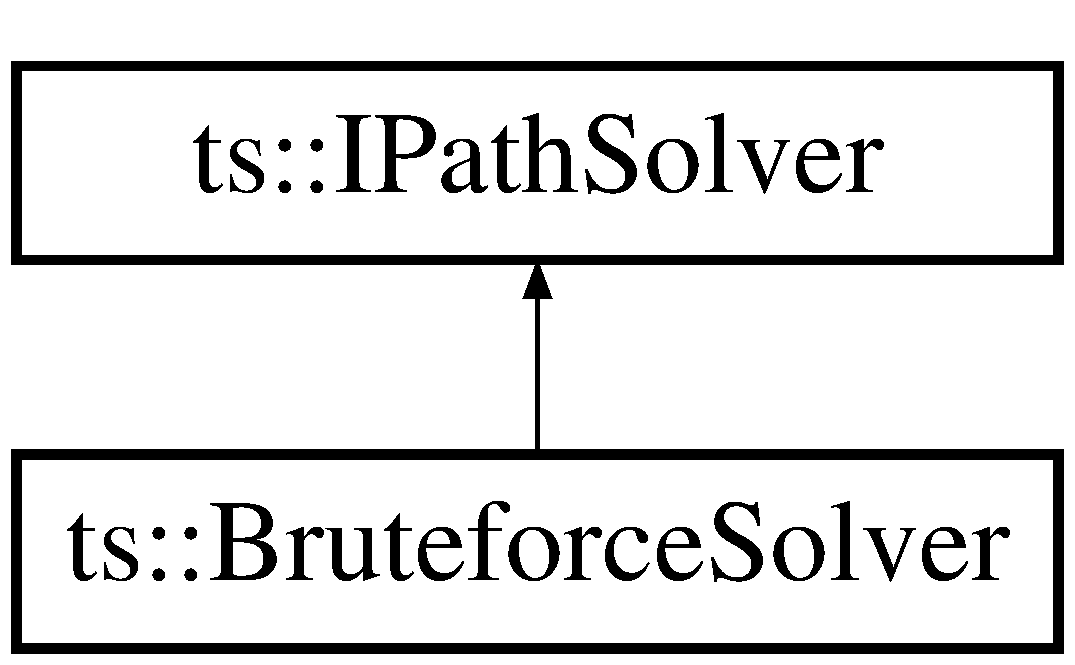
\includegraphics[height=2.000000cm]{classts_1_1_bruteforce_solver}
\end{center}
\end{figure}
\subsection*{Metody publiczne}
\begin{DoxyCompactItemize}
\item 
\mbox{\hyperlink{structts_1_1_solver_result}{Solver\+Result}} \mbox{\hyperlink{classts_1_1_bruteforce_solver_aeacf43058fd0498a2789ddcf091a42eb}{Solve}} (vector$<$ \mbox{\hyperlink{classts_1_1_city}{City}} $>$ cities, int start\+Index) override
\end{DoxyCompactItemize}


\subsection{Opis szczegółowy}
Klasa odpowiedzialna za szukanie drogi metoda siłową 

\subsection{Dokumentacja funkcji składowych}
\mbox{\Hypertarget{classts_1_1_bruteforce_solver_aeacf43058fd0498a2789ddcf091a42eb}\label{classts_1_1_bruteforce_solver_aeacf43058fd0498a2789ddcf091a42eb}} 
\index{ts\+::\+Bruteforce\+Solver@{ts\+::\+Bruteforce\+Solver}!Solve@{Solve}}
\index{Solve@{Solve}!ts\+::\+Bruteforce\+Solver@{ts\+::\+Bruteforce\+Solver}}
\subsubsection{\texorpdfstring{Solve()}{Solve()}}
{\footnotesize\ttfamily \mbox{\hyperlink{structts_1_1_solver_result}{Solver\+Result}} ts\+::\+Bruteforce\+Solver\+::\+Solve (\begin{DoxyParamCaption}\item[{vector$<$ \mbox{\hyperlink{classts_1_1_city}{City}} $>$}]{cities,  }\item[{int}]{start\+Index }\end{DoxyParamCaption})\hspace{0.3cm}{\ttfamily [override]}, {\ttfamily [virtual]}}

Metoda rozpoczyna algorytm brute force, odpowiada za liczenie czasu oraz ilosci permutacji


\begin{DoxyParams}{Parametry}
{\em cities} & vector przechowujacy miasta \\
\hline
{\em start\+Index} & zmienna przechowujaca index miasta, od ktorego nalezy zaczac \\
\hline
\end{DoxyParams}


Implementuje \mbox{\hyperlink{classts_1_1_i_path_solver_a3d76684ac8ebf47a5edb3af4e0280811}{ts\+::\+I\+Path\+Solver}}.



Dokumentacja dla tej klasy została wygenerowana z pliku\+:\begin{DoxyCompactItemize}
\item 
headers/\mbox{\hyperlink{_bruteforce_solver_8h}{Bruteforce\+Solver.\+h}}\end{DoxyCompactItemize}

\hypertarget{classts_1_1_city}{}\section{Dokumentacja klasy ts\+:\+:City}
\label{classts_1_1_city}\index{ts\+::\+City@{ts\+::\+City}}


{\ttfamily \#include $<$City.\+h$>$}

\subsection*{Atrybuty publiczne}
\begin{DoxyCompactItemize}
\item 
\mbox{\hyperlink{classts_1_1_point}{Point}} \mbox{\hyperlink{classts_1_1_city_abf6203580c06f5a20ab9fb1f374a386e}{location}}
\item 
string \mbox{\hyperlink{classts_1_1_city_ab0c6d6476ba2090fdfe254a8cfb55dd5}{name}}
\end{DoxyCompactItemize}


\subsection{Opis szczegółowy}
Klasa opisujaca miasto 

\subsection{Dokumentacja atrybutów składowych}
\mbox{\Hypertarget{classts_1_1_city_abf6203580c06f5a20ab9fb1f374a386e}\label{classts_1_1_city_abf6203580c06f5a20ab9fb1f374a386e}} 
\index{ts\+::\+City@{ts\+::\+City}!location@{location}}
\index{location@{location}!ts\+::\+City@{ts\+::\+City}}
\subsubsection{\texorpdfstring{location}{location}}
{\footnotesize\ttfamily \mbox{\hyperlink{classts_1_1_point}{Point}} ts\+::\+City\+::location}

location obiekt przechowujacy wspolrzedne miasta \mbox{\Hypertarget{classts_1_1_city_ab0c6d6476ba2090fdfe254a8cfb55dd5}\label{classts_1_1_city_ab0c6d6476ba2090fdfe254a8cfb55dd5}} 
\index{ts\+::\+City@{ts\+::\+City}!name@{name}}
\index{name@{name}!ts\+::\+City@{ts\+::\+City}}
\subsubsection{\texorpdfstring{name}{name}}
{\footnotesize\ttfamily string ts\+::\+City\+::name}

name pole przechowujace nazwe miasta 

Dokumentacja dla tej klasy została wygenerowana z pliku\+:\begin{DoxyCompactItemize}
\item 
headers/\mbox{\hyperlink{_city_8h}{City.\+h}}\end{DoxyCompactItemize}

\hypertarget{classts_1_1_city_seed}{}\section{Dokumentacja klasy ts\+:\+:City\+Seed}
\label{classts_1_1_city_seed}\index{ts\+::\+City\+Seed@{ts\+::\+City\+Seed}}


{\ttfamily \#include $<$City\+Seed.\+h$>$}

\subsection*{Metody publiczne}
\begin{DoxyCompactItemize}
\item 
vector$<$ \mbox{\hyperlink{classts_1_1_city}{City}} $>$ \mbox{\hyperlink{classts_1_1_city_seed_a3745be32ad7eae220cbbe5a0a2746aa1}{Seed\+Data}} (int count)
\end{DoxyCompactItemize}


\subsection{Opis szczegółowy}
Klasa odpowiedzialna za stworzenie obiektów typu \mbox{\hyperlink{classts_1_1_city}{City}} 

\subsection{Dokumentacja funkcji składowych}
\mbox{\Hypertarget{classts_1_1_city_seed_a3745be32ad7eae220cbbe5a0a2746aa1}\label{classts_1_1_city_seed_a3745be32ad7eae220cbbe5a0a2746aa1}} 
\index{ts\+::\+City\+Seed@{ts\+::\+City\+Seed}!Seed\+Data@{Seed\+Data}}
\index{Seed\+Data@{Seed\+Data}!ts\+::\+City\+Seed@{ts\+::\+City\+Seed}}
\subsubsection{\texorpdfstring{Seed\+Data()}{SeedData()}}
{\footnotesize\ttfamily vector$<$\mbox{\hyperlink{classts_1_1_city}{City}}$>$ ts\+::\+City\+Seed\+::\+Seed\+Data (\begin{DoxyParamCaption}\item[{int}]{count }\end{DoxyParamCaption})}

Metoda tworząca obiekty typu \mbox{\hyperlink{classts_1_1_city}{City}}


\begin{DoxyParams}{Parametry}
{\em count} & ilość miast \\
\hline
\end{DoxyParams}
\begin{DoxyReturn}{Zwraca}
vector$<$\+City$>$ 
\end{DoxyReturn}


Dokumentacja dla tej klasy została wygenerowana z pliku\+:\begin{DoxyCompactItemize}
\item 
headers/\mbox{\hyperlink{_city_seed_8h}{City\+Seed.\+h}}\end{DoxyCompactItemize}

\hypertarget{classts_1_1_drawer}{}\section{Dokumentacja klasy ts\+:\+:Drawer}
\label{classts_1_1_drawer}\index{ts\+::\+Drawer@{ts\+::\+Drawer}}


{\ttfamily \#include $<$Drawer.\+h$>$}

\subsection*{Metody publiczne}
\begin{DoxyCompactItemize}
\item 
\mbox{\hyperlink{classts_1_1_drawer_abe6a9094f9cf324006e30a7355adb15e}{Drawer}} (vector$<$ \mbox{\hyperlink{classts_1_1_city}{City}} $>$ cities)
\item 
void \mbox{\hyperlink{classts_1_1_drawer_a746a12f5e8693ea4aca8db7b91e89b32}{draw\+Cities}} ()
\item 
void \mbox{\hyperlink{classts_1_1_drawer_a5df30e090e866aca17986fbd5e518fc3}{draw\+Path}} ()
\end{DoxyCompactItemize}


\subsection{Opis szczegółowy}
Klasa odpowiedzialna za wyświetlanie na ekranie 

\subsection{Dokumentacja konstruktora i destruktora}
\mbox{\Hypertarget{classts_1_1_drawer_abe6a9094f9cf324006e30a7355adb15e}\label{classts_1_1_drawer_abe6a9094f9cf324006e30a7355adb15e}} 
\index{ts\+::\+Drawer@{ts\+::\+Drawer}!Drawer@{Drawer}}
\index{Drawer@{Drawer}!ts\+::\+Drawer@{ts\+::\+Drawer}}
\subsubsection{\texorpdfstring{Drawer()}{Drawer()}}
{\footnotesize\ttfamily ts\+::\+Drawer\+::\+Drawer (\begin{DoxyParamCaption}\item[{vector$<$ \mbox{\hyperlink{classts_1_1_city}{City}} $>$}]{cities }\end{DoxyParamCaption})}

Konstruktor klasy


\begin{DoxyParams}{Parametry}
{\em cities} & vector miast \\
\hline
\end{DoxyParams}


\subsection{Dokumentacja funkcji składowych}
\mbox{\Hypertarget{classts_1_1_drawer_a746a12f5e8693ea4aca8db7b91e89b32}\label{classts_1_1_drawer_a746a12f5e8693ea4aca8db7b91e89b32}} 
\index{ts\+::\+Drawer@{ts\+::\+Drawer}!draw\+Cities@{draw\+Cities}}
\index{draw\+Cities@{draw\+Cities}!ts\+::\+Drawer@{ts\+::\+Drawer}}
\subsubsection{\texorpdfstring{draw\+Cities()}{drawCities()}}
{\footnotesize\ttfamily void ts\+::\+Drawer\+::draw\+Cities (\begin{DoxyParamCaption}{ }\end{DoxyParamCaption})}

Metoda odpowiedzialna za wyświetlanie miast \mbox{\Hypertarget{classts_1_1_drawer_a5df30e090e866aca17986fbd5e518fc3}\label{classts_1_1_drawer_a5df30e090e866aca17986fbd5e518fc3}} 
\index{ts\+::\+Drawer@{ts\+::\+Drawer}!draw\+Path@{draw\+Path}}
\index{draw\+Path@{draw\+Path}!ts\+::\+Drawer@{ts\+::\+Drawer}}
\subsubsection{\texorpdfstring{draw\+Path()}{drawPath()}}
{\footnotesize\ttfamily void ts\+::\+Drawer\+::draw\+Path (\begin{DoxyParamCaption}{ }\end{DoxyParamCaption})}

Metoda odpowiedzialna za rysowanie drog 

Dokumentacja dla tej klasy została wygenerowana z pliku\+:\begin{DoxyCompactItemize}
\item 
headers/\mbox{\hyperlink{_drawer_8h}{Drawer.\+h}}\end{DoxyCompactItemize}

\hypertarget{classts_1_1_greedy_solver}{}\section{Dokumentacja klasy ts\+:\+:Greedy\+Solver}
\label{classts_1_1_greedy_solver}\index{ts\+::\+Greedy\+Solver@{ts\+::\+Greedy\+Solver}}


{\ttfamily \#include $<$Greedy\+Solver.\+h$>$}

Diagram dziedziczenia dla ts\+:\+:Greedy\+Solver\begin{figure}[H]
\begin{center}
\leavevmode
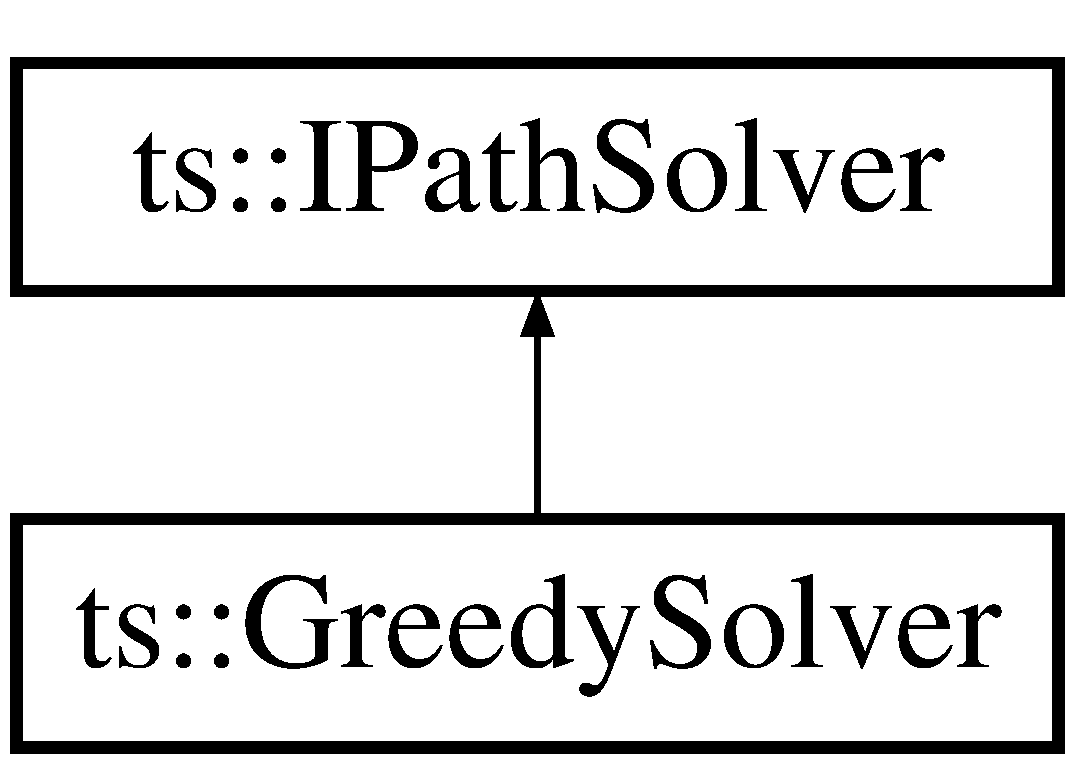
\includegraphics[height=2.000000cm]{classts_1_1_greedy_solver}
\end{center}
\end{figure}
\subsection*{Metody publiczne}
\begin{DoxyCompactItemize}
\item 
\mbox{\hyperlink{structts_1_1_solver_result}{Solver\+Result}} \mbox{\hyperlink{classts_1_1_greedy_solver_aa529740e0eaaadcd725e0ce23a34542f}{Solve}} (vector$<$ \mbox{\hyperlink{classts_1_1_city}{City}} $>$ cities, int start\+Index) override
\end{DoxyCompactItemize}


\subsection{Opis szczegółowy}
Klasa odpowiedzialna za szukanie drogi metoda Greedy 

\subsection{Dokumentacja funkcji składowych}
\mbox{\Hypertarget{classts_1_1_greedy_solver_aa529740e0eaaadcd725e0ce23a34542f}\label{classts_1_1_greedy_solver_aa529740e0eaaadcd725e0ce23a34542f}} 
\index{ts\+::\+Greedy\+Solver@{ts\+::\+Greedy\+Solver}!Solve@{Solve}}
\index{Solve@{Solve}!ts\+::\+Greedy\+Solver@{ts\+::\+Greedy\+Solver}}
\subsubsection{\texorpdfstring{Solve()}{Solve()}}
{\footnotesize\ttfamily \mbox{\hyperlink{structts_1_1_solver_result}{Solver\+Result}} ts\+::\+Greedy\+Solver\+::\+Solve (\begin{DoxyParamCaption}\item[{vector$<$ \mbox{\hyperlink{classts_1_1_city}{City}} $>$}]{cities,  }\item[{int}]{start\+Index }\end{DoxyParamCaption})\hspace{0.3cm}{\ttfamily [override]}, {\ttfamily [virtual]}}

Metoda sortuje vector


\begin{DoxyParams}{Parametry}
{\em cities} & \\
\hline
{\em start\+Index} & \\
\hline
\end{DoxyParams}
\begin{DoxyReturn}{Zwraca}

\end{DoxyReturn}


Implementuje \mbox{\hyperlink{classts_1_1_i_path_solver_a3d76684ac8ebf47a5edb3af4e0280811}{ts\+::\+I\+Path\+Solver}}.



Dokumentacja dla tej klasy została wygenerowana z pliku\+:\begin{DoxyCompactItemize}
\item 
headers/\mbox{\hyperlink{_greedy_solver_8h}{Greedy\+Solver.\+h}}\end{DoxyCompactItemize}

\hypertarget{classts_1_1_i_path_solver}{}\section{Dokumentacja klasy ts\+:\+:I\+Path\+Solver}
\label{classts_1_1_i_path_solver}\index{ts\+::\+I\+Path\+Solver@{ts\+::\+I\+Path\+Solver}}


{\ttfamily \#include $<$I\+Path\+Solver.\+h$>$}

Diagram dziedziczenia dla ts\+:\+:I\+Path\+Solver\begin{figure}[H]
\begin{center}
\leavevmode
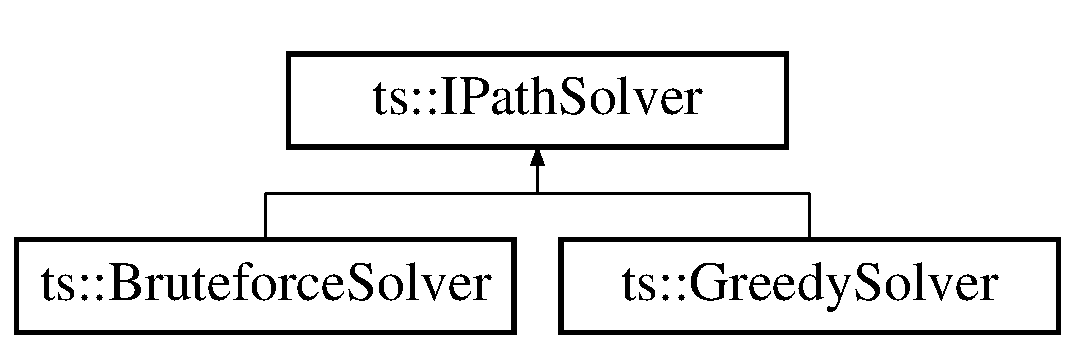
\includegraphics[height=2.000000cm]{classts_1_1_i_path_solver}
\end{center}
\end{figure}
\subsection*{Metody publiczne}
\begin{DoxyCompactItemize}
\item 
virtual \mbox{\hyperlink{structts_1_1_solver_result}{Solver\+Result}} \mbox{\hyperlink{classts_1_1_i_path_solver_a3d76684ac8ebf47a5edb3af4e0280811}{Solve}} (vector$<$ \mbox{\hyperlink{classts_1_1_city}{City}} $>$ cities, int start\+Index)=0
\end{DoxyCompactItemize}


\subsection{Opis szczegółowy}
Interfejs bazowy do definiowania swoich implementacji wyznaczania cyklu hamiltona 

\subsection{Dokumentacja funkcji składowych}
\mbox{\Hypertarget{classts_1_1_i_path_solver_a3d76684ac8ebf47a5edb3af4e0280811}\label{classts_1_1_i_path_solver_a3d76684ac8ebf47a5edb3af4e0280811}} 
\index{ts\+::\+I\+Path\+Solver@{ts\+::\+I\+Path\+Solver}!Solve@{Solve}}
\index{Solve@{Solve}!ts\+::\+I\+Path\+Solver@{ts\+::\+I\+Path\+Solver}}
\subsubsection{\texorpdfstring{Solve()}{Solve()}}
{\footnotesize\ttfamily virtual \mbox{\hyperlink{structts_1_1_solver_result}{Solver\+Result}} ts\+::\+I\+Path\+Solver\+::\+Solve (\begin{DoxyParamCaption}\item[{vector$<$ \mbox{\hyperlink{classts_1_1_city}{City}} $>$}]{cities,  }\item[{int}]{start\+Index }\end{DoxyParamCaption})\hspace{0.3cm}{\ttfamily [pure virtual]}}

Metoda wyznaczajaca cykl hamiltona


\begin{DoxyParams}{Parametry}
{\em cities} & vector miast \\
\hline
{\em start\+Index} & zmienna przechowujaca index miasta, od ktorego nalezy zaczac \\
\hline
\end{DoxyParams}
\begin{DoxyReturn}{Zwraca}

\end{DoxyReturn}


Implementowany w \mbox{\hyperlink{classts_1_1_greedy_solver_aa529740e0eaaadcd725e0ce23a34542f}{ts\+::\+Greedy\+Solver}} i \mbox{\hyperlink{classts_1_1_bruteforce_solver_aeacf43058fd0498a2789ddcf091a42eb}{ts\+::\+Bruteforce\+Solver}}.



Dokumentacja dla tej klasy została wygenerowana z pliku\+:\begin{DoxyCompactItemize}
\item 
headers/\mbox{\hyperlink{_i_path_solver_8h}{I\+Path\+Solver.\+h}}\end{DoxyCompactItemize}

\hypertarget{classts_1_1_point}{}\section{Dokumentacja klasy ts\+:\+:Point}
\label{classts_1_1_point}\index{ts\+::\+Point@{ts\+::\+Point}}


{\ttfamily \#include $<$Point.\+h$>$}

\subsection*{Metody publiczne}
\begin{DoxyCompactItemize}
\item 
double \mbox{\hyperlink{classts_1_1_point_acd9591fcf2e8df803d9713d075e13f42}{Get\+Distance\+To}} (\mbox{\hyperlink{classts_1_1_point}{Point}} other)
\end{DoxyCompactItemize}
\subsection*{Atrybuty publiczne}
\begin{DoxyCompactItemize}
\item 
double \mbox{\hyperlink{classts_1_1_point_ad726f45d332a723ab835926fec22e8b3}{x}}
\item 
double \mbox{\hyperlink{classts_1_1_point_aebe1d290b7b7dac45ac36a42157e5678}{y}}
\end{DoxyCompactItemize}


\subsection{Opis szczegółowy}
Klasa opisujaca punkt na ekranie 

\subsection{Dokumentacja funkcji składowych}
\mbox{\Hypertarget{classts_1_1_point_acd9591fcf2e8df803d9713d075e13f42}\label{classts_1_1_point_acd9591fcf2e8df803d9713d075e13f42}} 
\index{ts\+::\+Point@{ts\+::\+Point}!Get\+Distance\+To@{Get\+Distance\+To}}
\index{Get\+Distance\+To@{Get\+Distance\+To}!ts\+::\+Point@{ts\+::\+Point}}
\subsubsection{\texorpdfstring{Get\+Distance\+To()}{GetDistanceTo()}}
{\footnotesize\ttfamily double ts\+::\+Point\+::\+Get\+Distance\+To (\begin{DoxyParamCaption}\item[{\mbox{\hyperlink{classts_1_1_point}{Point}}}]{other }\end{DoxyParamCaption})}

Klasa liczaca odleglosc do innego punktu na ekranie


\begin{DoxyParams}{Parametry}
{\em other} & punkt, do ktorego ma byc zmierzona odleglosc \\
\hline
\end{DoxyParams}
\begin{DoxyReturn}{Zwraca}
odleglosc do punktu 
\end{DoxyReturn}


\subsection{Dokumentacja atrybutów składowych}
\mbox{\Hypertarget{classts_1_1_point_ad726f45d332a723ab835926fec22e8b3}\label{classts_1_1_point_ad726f45d332a723ab835926fec22e8b3}} 
\index{ts\+::\+Point@{ts\+::\+Point}!x@{x}}
\index{x@{x}!ts\+::\+Point@{ts\+::\+Point}}
\subsubsection{\texorpdfstring{x}{x}}
{\footnotesize\ttfamily double ts\+::\+Point\+::x}

x wspolrzedna x \mbox{\Hypertarget{classts_1_1_point_aebe1d290b7b7dac45ac36a42157e5678}\label{classts_1_1_point_aebe1d290b7b7dac45ac36a42157e5678}} 
\index{ts\+::\+Point@{ts\+::\+Point}!y@{y}}
\index{y@{y}!ts\+::\+Point@{ts\+::\+Point}}
\subsubsection{\texorpdfstring{y}{y}}
{\footnotesize\ttfamily double ts\+::\+Point\+::y}

y wspolrzedna y 

Dokumentacja dla tej klasy została wygenerowana z pliku\+:\begin{DoxyCompactItemize}
\item 
headers/\mbox{\hyperlink{_point_8h}{Point.\+h}}\end{DoxyCompactItemize}

\hypertarget{structts_1_1_solver_result}{}\section{Dokumentacja struktury ts\+:\+:Solver\+Result}
\label{structts_1_1_solver_result}\index{ts\+::\+Solver\+Result@{ts\+::\+Solver\+Result}}


{\ttfamily \#include $<$Solver\+Result.\+h$>$}

\subsection*{Atrybuty publiczne}
\begin{DoxyCompactItemize}
\item 
vector$<$ \mbox{\hyperlink{classts_1_1_city}{City}} $>$ \mbox{\hyperlink{structts_1_1_solver_result_aa6bbb18c7846f641eda9c690e833aedd}{result}}
\item 
time\+\_\+t \mbox{\hyperlink{structts_1_1_solver_result_a67b394211ddb67c3350920de2596fecf}{time}}
\item 
unsigned long long int \mbox{\hyperlink{structts_1_1_solver_result_ab284eb0df37ea9d104e2a1fbf918f518}{permutation\+Count}}
\end{DoxyCompactItemize}


\subsection{Opis szczegółowy}
Struktura opisujaca wynik dzialania algorytmow szukajacych drogi 

\subsection{Dokumentacja atrybutów składowych}
\mbox{\Hypertarget{structts_1_1_solver_result_ab284eb0df37ea9d104e2a1fbf918f518}\label{structts_1_1_solver_result_ab284eb0df37ea9d104e2a1fbf918f518}} 
\index{ts\+::\+Solver\+Result@{ts\+::\+Solver\+Result}!permutation\+Count@{permutation\+Count}}
\index{permutation\+Count@{permutation\+Count}!ts\+::\+Solver\+Result@{ts\+::\+Solver\+Result}}
\subsubsection{\texorpdfstring{permutation\+Count}{permutationCount}}
{\footnotesize\ttfamily unsigned long long int ts\+::\+Solver\+Result\+::permutation\+Count}

permutation\+Count przechowuje ilość permutacji \mbox{\Hypertarget{structts_1_1_solver_result_aa6bbb18c7846f641eda9c690e833aedd}\label{structts_1_1_solver_result_aa6bbb18c7846f641eda9c690e833aedd}} 
\index{ts\+::\+Solver\+Result@{ts\+::\+Solver\+Result}!result@{result}}
\index{result@{result}!ts\+::\+Solver\+Result@{ts\+::\+Solver\+Result}}
\subsubsection{\texorpdfstring{result}{result}}
{\footnotesize\ttfamily vector$<$\mbox{\hyperlink{classts_1_1_city}{City}}$>$ ts\+::\+Solver\+Result\+::result}

result przechowuje vector uporzadkowanych miast \mbox{\Hypertarget{structts_1_1_solver_result_a67b394211ddb67c3350920de2596fecf}\label{structts_1_1_solver_result_a67b394211ddb67c3350920de2596fecf}} 
\index{ts\+::\+Solver\+Result@{ts\+::\+Solver\+Result}!time@{time}}
\index{time@{time}!ts\+::\+Solver\+Result@{ts\+::\+Solver\+Result}}
\subsubsection{\texorpdfstring{time}{time}}
{\footnotesize\ttfamily time\+\_\+t ts\+::\+Solver\+Result\+::time}

time przechowuje czas dzialania algorytmu 

Dokumentacja dla tej struktury została wygenerowana z pliku\+:\begin{DoxyCompactItemize}
\item 
headers/\mbox{\hyperlink{_solver_result_8h}{Solver\+Result.\+h}}\end{DoxyCompactItemize}

\chapter{Dokumentacja plików}
\hypertarget{_bruteforce_solver_8h}{}\section{Dokumentacja pliku headers/\+Bruteforce\+Solver.h}
\label{_bruteforce_solver_8h}\index{headers/\+Bruteforce\+Solver.\+h@{headers/\+Bruteforce\+Solver.\+h}}
{\ttfamily \#include \char`\"{}I\+Path\+Solver.\+h\char`\"{}}\newline
\subsection*{Komponenty}
\begin{DoxyCompactItemize}
\item 
class \mbox{\hyperlink{classts_1_1_bruteforce_solver}{ts\+::\+Bruteforce\+Solver}}
\end{DoxyCompactItemize}
\subsection*{Przestrzenie nazw}
\begin{DoxyCompactItemize}
\item 
 \mbox{\hyperlink{namespacets}{ts}}
\end{DoxyCompactItemize}

\hypertarget{_city_8h}{}\section{Dokumentacja pliku headers/\+City.h}
\label{_city_8h}\index{headers/\+City.\+h@{headers/\+City.\+h}}
{\ttfamily \#include $<$string$>$}\newline
{\ttfamily \#include \char`\"{}Point.\+h\char`\"{}}\newline
\subsection*{Komponenty}
\begin{DoxyCompactItemize}
\item 
class \mbox{\hyperlink{classts_1_1_city}{ts\+::\+City}}
\end{DoxyCompactItemize}
\subsection*{Przestrzenie nazw}
\begin{DoxyCompactItemize}
\item 
 \mbox{\hyperlink{namespacets}{ts}}
\end{DoxyCompactItemize}

\hypertarget{_city_seed_8h}{}\section{Dokumentacja pliku headers/\+City\+Seed.h}
\label{_city_seed_8h}\index{headers/\+City\+Seed.\+h@{headers/\+City\+Seed.\+h}}
{\ttfamily \#include $<$vector$>$}\newline
{\ttfamily \#include \char`\"{}../headers/\+City.\+h\char`\"{}}\newline
\subsection*{Komponenty}
\begin{DoxyCompactItemize}
\item 
class \mbox{\hyperlink{classts_1_1_city_seed}{ts\+::\+City\+Seed}}
\end{DoxyCompactItemize}
\subsection*{Przestrzenie nazw}
\begin{DoxyCompactItemize}
\item 
 \mbox{\hyperlink{namespacets}{ts}}
\end{DoxyCompactItemize}

\hypertarget{_drawer_8h}{}\section{Dokumentacja pliku headers/\+Drawer.h}
\label{_drawer_8h}\index{headers/\+Drawer.\+h@{headers/\+Drawer.\+h}}
{\ttfamily \#include $<$iostream$>$}\newline
{\ttfamily \#include $<$G\+L/gl.\+h$>$}\newline
{\ttfamily \#include $<$unistd.\+h$>$}\newline
{\ttfamily \#include \char`\"{}../headers/\+City\+Seed.\+h\char`\"{}}\newline
\subsection*{Komponenty}
\begin{DoxyCompactItemize}
\item 
class \mbox{\hyperlink{classts_1_1_drawer}{ts\+::\+Drawer}}
\end{DoxyCompactItemize}
\subsection*{Przestrzenie nazw}
\begin{DoxyCompactItemize}
\item 
 \mbox{\hyperlink{namespacets}{ts}}
\end{DoxyCompactItemize}

\hypertarget{_greedy_solver_8h}{}\section{Dokumentacja pliku headers/\+Greedy\+Solver.h}
\label{_greedy_solver_8h}\index{headers/\+Greedy\+Solver.\+h@{headers/\+Greedy\+Solver.\+h}}
{\ttfamily \#include \char`\"{}I\+Path\+Solver.\+h\char`\"{}}\newline
\subsection*{Komponenty}
\begin{DoxyCompactItemize}
\item 
class \mbox{\hyperlink{classts_1_1_greedy_solver}{ts\+::\+Greedy\+Solver}}
\end{DoxyCompactItemize}
\subsection*{Przestrzenie nazw}
\begin{DoxyCompactItemize}
\item 
 \mbox{\hyperlink{namespacets}{ts}}
\end{DoxyCompactItemize}

\hypertarget{_i_path_solver_8h}{}\section{Dokumentacja pliku headers/\+I\+Path\+Solver.h}
\label{_i_path_solver_8h}\index{headers/\+I\+Path\+Solver.\+h@{headers/\+I\+Path\+Solver.\+h}}
{\ttfamily \#include \char`\"{}City.\+h\char`\"{}}\newline
{\ttfamily \#include \char`\"{}Solver\+Result.\+h\char`\"{}}\newline
{\ttfamily \#include $<$vector$>$}\newline
\subsection*{Komponenty}
\begin{DoxyCompactItemize}
\item 
class \mbox{\hyperlink{classts_1_1_i_path_solver}{ts\+::\+I\+Path\+Solver}}
\end{DoxyCompactItemize}
\subsection*{Przestrzenie nazw}
\begin{DoxyCompactItemize}
\item 
 \mbox{\hyperlink{namespacets}{ts}}
\end{DoxyCompactItemize}

\hypertarget{_point_8h}{}\section{Dokumentacja pliku headers/\+Point.h}
\label{_point_8h}\index{headers/\+Point.\+h@{headers/\+Point.\+h}}
\subsection*{Komponenty}
\begin{DoxyCompactItemize}
\item 
class \mbox{\hyperlink{classts_1_1_point}{ts\+::\+Point}}
\end{DoxyCompactItemize}
\subsection*{Przestrzenie nazw}
\begin{DoxyCompactItemize}
\item 
 \mbox{\hyperlink{namespacets}{ts}}
\end{DoxyCompactItemize}

\hypertarget{_solver_result_8h}{}\section{Dokumentacja pliku headers/\+Solver\+Result.h}
\label{_solver_result_8h}\index{headers/\+Solver\+Result.\+h@{headers/\+Solver\+Result.\+h}}
{\ttfamily \#include $<$vector$>$}\newline
{\ttfamily \#include \char`\"{}City.\+h\char`\"{}}\newline
\subsection*{Komponenty}
\begin{DoxyCompactItemize}
\item 
struct \mbox{\hyperlink{structts_1_1_solver_result}{ts\+::\+Solver\+Result}}
\end{DoxyCompactItemize}
\subsection*{Przestrzenie nazw}
\begin{DoxyCompactItemize}
\item 
 \mbox{\hyperlink{namespacets}{ts}}
\end{DoxyCompactItemize}

%--- End generated contents ---

% Index
\backmatter
\newpage
\phantomsection
\clearemptydoublepage
\addcontentsline{toc}{chapter}{Indeks}
\printindex

\end{document}
